\documentclass[border=8pt]{standalone}
\usepackage{pgfplots}
\usepgfplotslibrary{groupplots}
\pgfplotsset{compat=1.18}
\renewcommand{\familydefault}{\sfdefault}
\definecolor{oursline}{HTML}{00747C}
\definecolor{omleline}{HTML}{773588}
\definecolor{ink}{HTML}{17242D}
\definecolor{muted}{HTML}{4A5C67}
\definecolor{gridline}{HTML}{E3EAED}
\begin{document}
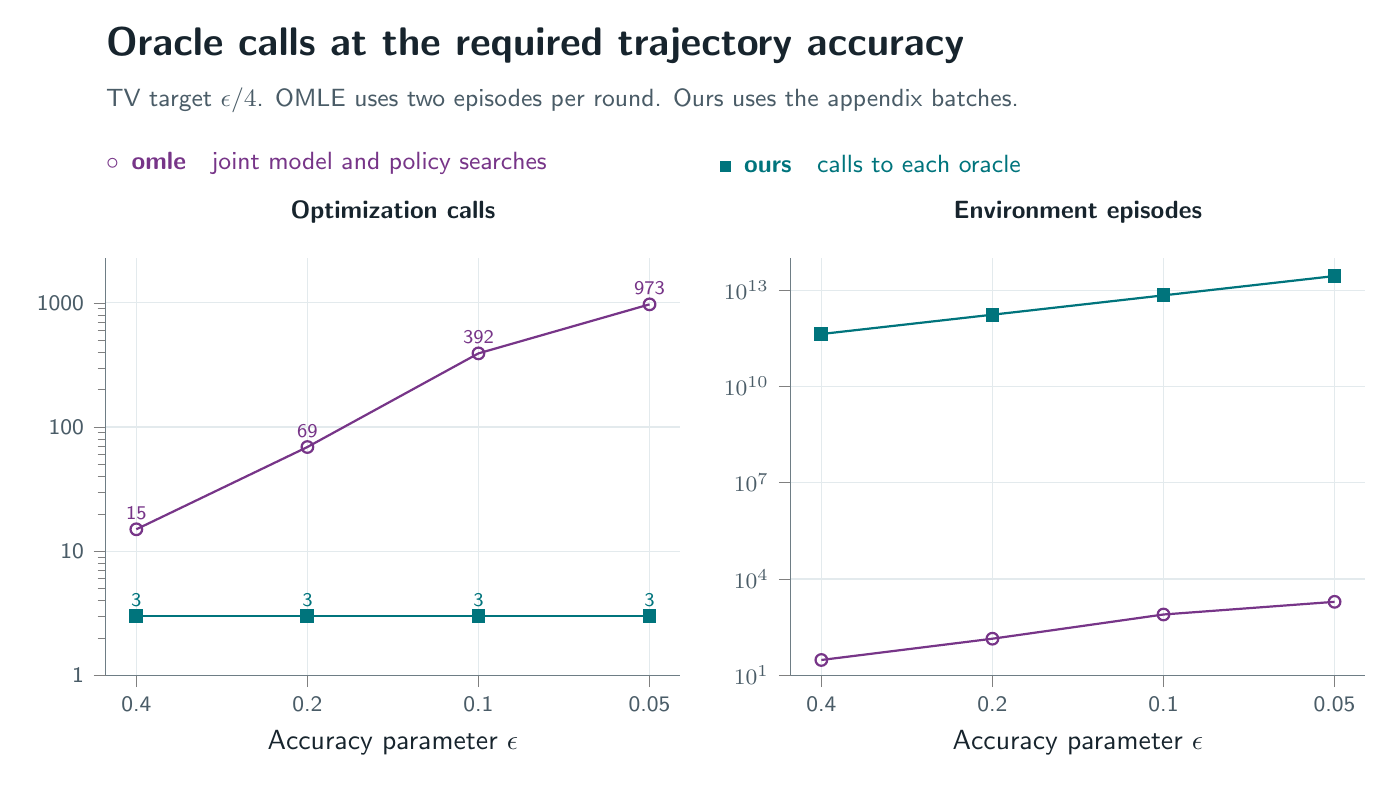
\begin{tikzpicture}[text=ink]
\begin{groupplot}[
  group style={group size=2 by 1,horizontal sep=1.4cm},
  width=7.3cm,height=5.3cm,scale only axis,
  xmin=-.18,xmax=3.18,xtick={0,1,2,3},ymode=log,
  axis lines*=left,axis line style={muted!80},
  tick align=outside,tick label style={font=\footnotesize,text=muted},
  title style={font=\small\bfseries,text=ink,yshift=1mm},
  grid=major,grid style={gridline},xlabel={Accuracy parameter $\epsilon$},
  clip=false,
]
\nextgroupplot[title={Optimization calls},xticklabels={0.4,0.2,0.1,0.05},ymin=1,ymax=2300,ytick={1,10,100,1000},yticklabels={1,10,100,1000}]
\addplot[omleline,thick,mark=o,mark size=2.1pt] coordinates {(0,15) (1,69) (2,392) (3,973)};
\node[anchor=south,font=\scriptsize,text=omleline] at (axis cs:0,15) {15};
\node[anchor=south,font=\scriptsize,text=omleline] at (axis cs:1,69) {69};
\node[anchor=south,font=\scriptsize,text=omleline] at (axis cs:2,392) {392};
\node[anchor=south,font=\scriptsize,text=omleline] at (axis cs:3,973) {973};
\addplot[oursline,thick,mark=square*,mark size=2.1pt] coordinates {(0,3) (1,3) (2,3) (3,3)};
\node[anchor=south,font=\scriptsize,text=oursline] at (axis cs:0,3) {3};
\node[anchor=south,font=\scriptsize,text=oursline] at (axis cs:1,3) {3};
\node[anchor=south,font=\scriptsize,text=oursline] at (axis cs:2,3) {3};
\node[anchor=south,font=\scriptsize,text=oursline] at (axis cs:3,3) {3};
\nextgroupplot[title={Environment episodes},xticklabels={0.4,0.2,0.1,0.05},ymin=10,ymax=1e14,ytick={10,1e4,1e7,1e10,1e13}]
\addplot[omleline,thick,mark=o,mark size=2.1pt] coordinates {(0,30) (1,138) (2,784) (3,1946)};
\addplot[oursline,thick,mark=square*,mark size=2.1pt] coordinates {(0,427648271078) (1,1710593084286) (2,6842372337134) (3,27369489348528)};
\end{groupplot}
\node[anchor=west,inner sep=0pt,font=\bfseries\Large] at ([yshift=27mm]group c1r1.north west) {Oracle calls at the required trajectory accuracy};
\node[anchor=west,inner sep=0pt,text=muted,font=\small] at ([yshift=20mm]group c1r1.north west) {TV target $\epsilon/4$. OMLE uses two episodes per round. Ours uses the appendix batches.};
\node[anchor=west,inner sep=0pt,text=omleline,font=\small] at ([yshift=12mm]group c1r1.north west) {$\circ$\enspace\textbf{omle}\quad joint model and policy searches};
\node[anchor=west,inner sep=0pt,text=oursline,font=\small] at ([xshift=78mm,yshift=12mm]group c1r1.north west) {\rule{4pt}{4pt}\enspace\textbf{ours}\quad calls to each oracle};
\end{tikzpicture}
\end{document}
